\documentclass{article}
\usepackage[T1]{fontenc}
\usepackage{lmodern}
\usepackage{graphicx}
\usepackage{amsmath,amssymb}
\usepackage[a4paper,margin=2cm]{geometry}
\usepackage[absolute,overlay]{textpos}
\setlength{\TPHorizModule}{1mm}
\setlength{\TPVertModule}{1mm}
\usepackage[indonesian]{babel}
\usepackage{hyperref}
\setlength{\emergencystretch}{2em}
% unit: Halaman 2

\begin{document}

% === Halaman 2 (llm) ===

\section*{The Prisoner's Problem}

\begin{itemize}
    \item Diperkenalkan oleh Simmons -- 1983
    \item Dilakukan dalam konteks USA -- USSR nuclear non-proliferation treaty compliance checking
\end{itemize}

\vspace{60mm}

\textbf{Pesan rahasia: "malam ini kita kabur"}

% deskripsi: Ilustrasi konsep The Prisoner's Problem yang menampilkan tiga karakter: Alice dan Bob di dalam penjara, serta Wendy di antara mereka yang bertindak sebagai perantara pesan rahasia.
% bbox normalisasi: [0.2400, 0.4030, 0.6510, 0.8970]
\begin{textblock*}{86.31mm}(50.40mm,119.69mm)
\noindent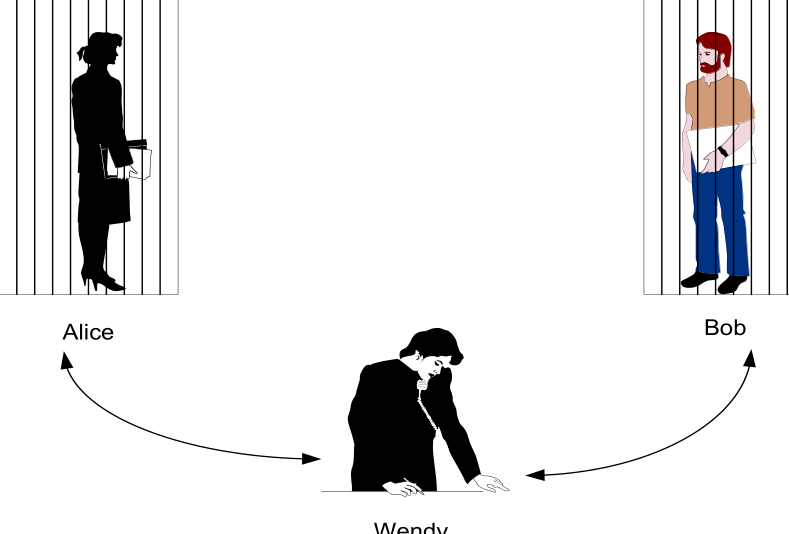
\includegraphics[width=86.31mm,height=146.72mm]{../../images/llm/page_002_img_01.png}%
\end{textblock*}

\end{document}
